% =====================================================================
%  Group 08 Technical Report
%  Short-Term Bitcoin Price Prediction from Live News Sentiment
%
%  Build:  pdflatex main && bibtex main && pdflatex main && pdflatex main
%          (or: latexmk -pdf main.tex). Works on Overleaf as is.
%
%  PRELIMINARY NUMBERS: every result from the first training run
%  (2026-11-28) is wrapped in \prelim{...} and every place that must be
%  refreshed after the final retrain is marked with \UPDATE{...}.
%  Search this file for "\prelim" and "\UPDATE" after the retrain.
%  Items the team must write themselves (names, IDs, contributions) are
%  marked \TOFILL{...}.
%  When everything is final, change \showupdatestrue to \showupdatesfalse
%  below: the highlights and notes then disappear from the PDF.
% =====================================================================
\documentclass[12pt,a4paper,oneside]{report}

\usepackage[T1]{fontenc}
\usepackage[utf8]{inputenc}
\usepackage{lmodern}
\usepackage[margin=2.5cm,headheight=15pt]{geometry}
\usepackage{amsmath,amssymb}
\usepackage{graphicx}
\usepackage{booktabs}
\usepackage{tabularx}
\usepackage{multirow}
\usepackage{longtable}
\usepackage{array}
\usepackage[table]{xcolor}
\usepackage{enumitem}
\usepackage{caption}
\usepackage{float}
\usepackage{listings}
\usepackage{tikz}
\usetikzlibrary{arrows.meta,positioning,fit,calc}
\usepackage[numbers,sort&compress]{natbib}
\usepackage{titlesec}
\usepackage{fancyhdr}
\usepackage[hidelinks]{hyperref}

% ---------------------------------------------------------------------
%  Preliminary-result markers
% ---------------------------------------------------------------------
\newif\ifshowupdates
\showupdatestrue   % <- set to \showupdatesfalse for the final version
\ifshowupdates
  \newcommand{\prelim}[1]{\colorbox{yellow!40}{#1}}
  \newcommand{\TOFILL}[1]{\par\noindent\fcolorbox{blue!60!black}{blue!5}{%
    \parbox{\dimexpr\linewidth-2\fboxsep-2\fboxrule}{\small\textbf{\textcolor{blue!60!black}{TO FILL IN:}} #1}}\par\medskip}
  \newcommand{\UPDATE}[1]{\par\noindent\fcolorbox{red!70!black}{red!6}{%
    \parbox{\dimexpr\linewidth-2\fboxsep-2\fboxrule}{\small\textbf{\textcolor{red!70!black}{UPDATE AFTER FINAL RETRAIN:}} #1}}\par\medskip}
\else
  \newcommand{\prelim}[1]{#1}
  \newcommand{\UPDATE}[1]{}
  \newcommand{\TOFILL}[1]{}
\fi

\newcommand{\code}[1]{\texttt{\detokenize{#1}}}
\newcommand{\Wobs}{W_{\mathrm{obs}}}
\newcommand{\Wlag}{W_{\mathrm{lag}}}
\newcommand{\Wpred}{W_{\mathrm{pred}}}
\newcommand{\dobs}{\Delta_{\mathrm{obs}}}
\newcommand{\dlag}{\Delta_{\mathrm{lag}}}
\newcommand{\dpred}{\Delta_{\mathrm{pred}}}

\titleformat{\chapter}[block]{\normalfont\LARGE\bfseries\raggedright}{CHAPTER \thechapter.}{0.6em}{\MakeUppercase}
\titlespacing*{\chapter}{0pt}{-10pt}{18pt}

\pagestyle{fancy}
\fancyhf{}
\fancyhead[L]{\small\nouppercase{\leftmark}}
\fancyfoot[C]{\thepage}
\renewcommand{\headrulewidth}{0.4pt}

\lstset{
  basicstyle=\ttfamily\footnotesize,
  breaklines=true,
  frame=single,
  numbers=left,
  numberstyle=\tiny\color{gray},
  columns=fullflexible,
  keepspaces=true,
  showstringspaces=false,
}

\setlist{itemsep=2pt,topsep=4pt}
\renewcommand{\arraystretch}{1.15}
\newcolumntype{Y}{>{\raggedright\arraybackslash}X}

\begin{document}

% =====================================================================
%  Title page
% =====================================================================
\begin{titlepage}
  \centering
  {\large \TOFILL{University, faculty and course name, course code, lecturer.}}
  \vspace*{1.5cm}

  {\Large\bfseries WEB MINING\par}
  \vspace{0.6cm}
  {\large Technical Report -- Group 08\par}
  \vspace{2cm}

  {\LARGE\bfseries Short-Term Bitcoin Price Prediction\\[4pt] from Live News Sentiment\par}
  \vspace{0.6cm}
  {\large An end-to-end web mining pipeline with LLM sentiment scoring,\\
   leakage-safe evaluation and a streaming architecture\par}
  \vspace{2.5cm}

  \TOFILL{Fill in every member.}
  \begin{tabular}{ll}
    \toprule
    \textbf{Member} & \textbf{Student ID} \\
    \midrule
    Member 1 & ID \\
    Member 2 & ID \\
    Member 3 & ID \\
    Member 4 & ID \\
    \bottomrule
  \end{tabular}

  \vfill
  {\large December 2026\par}
\end{titlepage}

% =====================================================================
%  Abstract
% =====================================================================
\pagenumbering{roman}
\chapter*{Abstract}
\addcontentsline{toc}{chapter}{Abstract}

We present an end-to-end web mining system that collects cryptocurrency news
in real time, scores every article with a large language model (LLM), and
uses the aggregated sentiment together with technical indicators to predict
the Bitcoin (BTC) price change over a 10-minute window. Full article text is
crawled every 10 minutes from CoinMarketCap and 30 RSS feeds, cleaned,
deduplicated and streamed through Apache Kafka to a sentiment service that
queries Google Gemini (\code{gemini-3.5-flash-lite}) for a label, a score in
$[-1,1]$ and a confidence. One-minute BTC/USDT candles come from Binance.
Apache Airflow orchestrates collection, scoring, daily retraining and live
prediction. MongoDB stores the data, MLflow tracks experiments, and a FastAPI
dashboard shows prices, news, sentiment and predictions.

Compared with the earlier version of this project, the dataset is built so
that no feature can see the future. A mandatory 10-minute lag separates the
news window from the target window, it is checked on every sample, and all
preprocessing is fitted inside each training fold. Models are chosen with
walk-forward cross-validation and an embargo, then tested once on a final
held-out period. On a first run with \prelim{282} samples built from
\prelim{1,868} Gemini-scored articles collected between 26 and 28 November
2026, a random forest using technical features alone reached a test
direction accuracy of \prelim{52\%}. Adding news features raised it to
\prelim{about 62\%}, and adding time-of-day features to \prelim{67\%}. The
information coefficient rose from \prelim{0.11} to \prelim{0.30--0.38}, while
$R^2$ stayed close to zero. With only \prelim{42} test samples, these
gains are encouraging but not yet statistically conclusive, and a
fee-aware trading rule made no trades. We therefore present the system as a
sound, reproducible framework for testing the news-sentiment hypothesis,
not as a trading strategy.

\UPDATE{Replace every highlighted number in the abstract with the final retrain results (Section~\ref{sec:results}).}

\tableofcontents
\listoffigures
\listoftables

\clearpage
\pagenumbering{arabic}

% =====================================================================
\chapter{Member Contribution}\label{ch:members}
% =====================================================================

\TOFILL{This chapter is for the team to fill in. The structure follows the original report. Replace the placeholders with each member's real name and work.}

\section{Project Leadership and Infrastructure}
\emph{Member name.} Overall coordination, system architecture, Docker Compose
stack (Kafka, MongoDB, Airflow, MLflow, FastAPI), deployment on the team's
machines.

\section{Data Acquisition and Preprocessing}
\emph{Member name.} CoinMarketCap crawler, RSS collector and feed health
checks, full-text extraction, deduplication, Binance price backfill.

\section{Machine Learning Model Development}
\emph{Member name.} Gemini sentiment scoring, NLP features, leakage-safe
dataset builder, model zoo, walk-forward evaluation.

\section{Evaluation and Documentation}
\emph{Member name.} Experiments, ablation study, sanity checks, dashboard,
this report.

\section{Shared Responsibilities}
Code review, testing (the repository has a unit and end-to-end test suite
run in continuous integration), data monitoring during the live collection
period.

\section{Contribution Summary Table}
\begin{table}[H]
  \centering
  \caption{Summary of individual contributions}
  \label{tab:contrib}
  \begin{tabularx}{\linewidth}{lYc}
    \toprule
    \textbf{Member} & \textbf{Main tasks} & \textbf{Share} \\
    \midrule
    Member 1 & Leadership, infrastructure & --\% \\
    Member 2 & Data acquisition, preprocessing & --\% \\
    Member 3 & Sentiment, features, models & --\% \\
    Member 4 & Evaluation, dashboard, report & --\% \\
    \bottomrule
  \end{tabularx}
\end{table}

% =====================================================================
\chapter{Introduction and Problem Definition}\label{ch:intro}
% =====================================================================

\section{Background}
The World Wide Web has grown from a static collection of documents into a
dynamic ecosystem in which news outlets, blogs and social platforms publish
a continuous stream of opinion. Web mining, the application of data mining
to web content, structure and usage, provides the techniques to turn this
unstructured stream into usable signals \citep{liu2012sentiment}.

The cryptocurrency market is a domain where such signals are thought to
matter. Bitcoin has no cash flows to anchor its value, trades around the
clock, and is widely reported to react to news, regulation and public
attention \citep{kristoufek2013bitcoin,garcia2015social}. Stories about
exchange-traded fund (ETF) flows, regulatory decisions, hacks or large
purchases can move the price within minutes. The volume and speed of this
news make manual analysis impossible, so the pipeline from crawling to
prediction has to be automated.

\section{Problem Statement}
Predicting short-term Bitcoin price movements from news is hard for several
reasons:
\begin{itemize}
  \item \textbf{Low signal-to-noise ratio.} Ten-minute returns are close to
        a random walk. Any predictable component is small compared with
        the noise \citep{fama1970efficient}.
  \item \textbf{Information overload.} Dozens of outlets publish hundreds of
        articles a day. Only a few of them matter for the price.
  \item \textbf{Unstructured text.} The signal is hidden in headlines and
        article bodies and must be converted into numeric features.
  \item \textbf{Semantic nuance.} Keyword methods miss context: ``BTC drops
        to a discount zone'' can be bullish, and promotional ``to the moon''
        pieces are not genuine optimism.
  \item \textbf{Evaluation pitfalls.} Overlapping windows, preprocessing
        fitted on the whole dataset, and news published inside the target
        window can all make a model look far better than it is
        \citep{lopezdeprado2018advances}.
\end{itemize}
This project builds and evaluates an automated pipeline from raw web news to
a price-direction forecast, with special care for the last point.

\section{Objectives}
The main objective is an end-to-end web mining system that uses news
sentiment to predict the 10-minute BTC price change. The sub-objectives are:
\begin{enumerate}
  \item \textbf{Web data collection.} Continuously crawl full-text crypto
        news from CoinMarketCap and 30 RSS feeds, and collect 1-minute BTC
        prices from Binance.
  \item \textbf{Information extraction and enrichment.} Score each article
        with an LLM (Gemini) for a label, a sentiment score and a
        confidence, and extract NLP features such as polarity, keywords and
        named entities.
  \item \textbf{Data mining and analysis.} Align sentiment with future
        price changes in a leakage-safe dataset, train ensemble models, and
        measure the value of news with a controlled ablation study.
  \item \textbf{System implementation.} Build a containerised streaming
        architecture (Docker, Airflow, Kafka, MongoDB, MLflow, FastAPI)
        that runs on a student laptop.
\end{enumerate}

\section{Scope of the Project}
\begin{itemize}
  \item \textbf{Target asset:} Bitcoin (BTC/USDT spot) only.
  \item \textbf{News sources:} CoinMarketCap news and 30 crypto-news RSS
        feeds, collected live from 26 November 2026. Historical news
        archives were not used (Section~\ref{sec:history}).
  \item \textbf{Price source:} Binance 1-minute candles, with 90 days
        backfilled.
  \item \textbf{Horizon:} 30-minute observation window, 10-minute lag and
        10-minute prediction window, sampled every 10 minutes.
  \item \textbf{Target:} percentage price change (regression), evaluated
        mainly by its sign (direction accuracy) and rank correlation
        (information coefficient).
  \item \textbf{Techniques:} Gemini 3.5 Flash-Lite for sentiment, ridge
        regression, random forest, gradient boosting and LightGBM for
        prediction.
\end{itemize}

% =====================================================================
\chapter{Literature Review and Problem Formulation}\label{ch:lit}
% =====================================================================

Sentiment analysis is the computational study of opinions, attitudes and
emotions in text \citep{liu2012sentiment}. In finance it aims to quantify
market psychology and link it to asset prices. This chapter reviews related
work and then formalises our approach, following the four-stage framework of
the original report.

\section{Related Work}\label{sec:related}
\paragraph{Sentiment and markets.} \citet{bollen2011twitter} reported that
public mood measured on Twitter helped predict daily moves of the Dow Jones
index. For Bitcoin, \citet{kristoufek2013bitcoin} found a two-way
relationship between price and search or Wikipedia attention, and
\citet{garcia2015social} showed that social-media signals could drive
profitable trading rules at daily frequency. \citet{abraham2018cryptocurrency}
found tweet volume to be a stronger predictor than tweet polarity, a pattern
we also look for in our feature importances.

\paragraph{From lexicons to language models.} Early financial sentiment
relied on dictionaries. General lexicons misclassify financial language, which
led to domain lexicons such as \citet{loughran2011liability}. VADER
\citep{hutto2014vader} is a rule-based method tuned for short social text and
is the basis of our offline fallback. Transformer models such as FinBERT
\citep{araci2019finbert} improved accuracy further, and recent work shows that
general-purpose LLMs can extract return-relevant signals from headlines with
zero-shot prompts \citep{lopezlira2023chatgpt}. We follow that direction with
Gemini.

\paragraph{Evaluation of financial models.} Financial time series are
non-stationary and serially dependent. Random train-test splits, overlapping
labels and preprocessing fitted on all data leak information and inflate
results. \citet{lopezdeprado2018advances} recommends purged, embargoed
cross-validation, which we adopt. We also report the information coefficient
(rank correlation between prediction and outcome), a standard measure of
forecasting skill in quantitative finance \citep{grinold2000active}.

\section{Problem Formulation and Temporal Framework}\label{sec:temporal}
\paragraph{Research question.} Does sentiment extracted from cryptocurrency
news contain information about the next 10-minute Bitcoin price change that
is not already in the price history?

\paragraph{Temporal structure.} For each decision time $t$ we define three
periods:
\begin{enumerate}
  \item Observation window $\Wobs = [t-\dobs,\, t)$, with $\dobs = 30$ min:
        news articles and candles used as features.
  \item Lag period $\Wlag = [t,\, t+\dlag)$, with $\dlag = 10$ min: never
        used, so that news cannot overlap the target.
  \item Prediction window $\Wpred = [t+\dlag,\, t+\dlag+\dpred]$, with
        $\dpred = 10$ min: the period whose price change is predicted.
\end{enumerate}
An article $d_i$ with publication time $\tau_i$ is used for decision time $t$
only if $t-\dobs \le \tau_i < t$. Price features use only candles that closed
by $t$.

\begin{figure}[H]
\centering
\begin{tikzpicture}[x=0.27cm,y=1cm,font=\small]
  \draw[-{Latex}] (0,0) -- (52,0) node[right]{time};
  \fill[blue!15]  (0,0.15) rectangle (30,0.85);
  \fill[gray!20]  (30,0.15) rectangle (40,0.85);
  \fill[orange!30](40,0.15) rectangle (50,0.85);
  \node at (15,0.5) {observation $\Wobs$ (30 min)};
  \node at (35,0.5) {lag};
  \node at (45,0.5) {target $\Wpred$};
  \foreach \x/\l in {0/{09:50},30/{10:20},40/{10:30},50/{10:40}}
    {\draw (\x,0.1) -- (\x,-0.1) node[below]{\l};}
  \node[below] at (30,-0.55) {$t$};
\end{tikzpicture}
\caption{Temporal framework for one sample with decision time $t=$ 10:20.}
\label{fig:timeline}
\end{figure}

\section{Stage 1: Sentiment Extraction from Individual Articles}
An LLM implements an extraction function
\begin{equation}
  \phi_{\mathrm{LLM}} : \mathcal{D} \to [-1,1] \times [0,1] \times \mathcal{C},
  \qquad (s_i, c_i, \ell_i) = \phi_{\mathrm{LLM}}(d_i;\, P),
\end{equation}
where $P$ is the prompt (Appendix~\ref{sec:prompt}), $s_i$ the sentiment
score (negative is bearish), $c_i$ the model's confidence, and
$\ell_i \in \mathcal{C} = \{\text{bullish}, \text{bearish},
\text{manipulation}, \text{neutral}\}$ the article's intent. The original
prompt only asked for a label and a confidence, so the score used by the
formulas below was undefined. Our prompt asks for all three explicitly and
enforces them with a JSON response schema.

\section{Stage 2: Temporal Aggregation}
Given the $N$ articles in $\Wobs$, the confidence-weighted market sentiment is
\begin{equation}
  S_{\mathrm{market}}(t) = \frac{\sum_{i=1}^{N} c_i\, s_i}{\sum_{i=1}^{N} c_i}.
\end{equation}
For example, articles with $(s,c)$ equal to $(0.85, 0.95)$, $(-0.30, 0.25)$
and $(0, 0.90)$ give $S_{\mathrm{market}} = 0.733/2.10 = 0.349$, while the
plain mean is $0.183$: the confident regulatory headline dominates.

We add a recency-weighted variant with a 10-minute half-life, so that the
newest news counts most:
\begin{equation}
  S_{\mathrm{decay}}(t) = \frac{\sum_i w_i c_i s_i}{\sum_i w_i c_i},
  \qquad w_i = 2^{-(t-\tau_i)/10\,\mathrm{min}}.
\end{equation}

\section{Stage 3: Feature Engineering}
The original seven-dimensional sentiment vector
$[N, \bar{s}, \sigma_s, \max s, \min s, N_{\mathrm{manip}}, \bar{c}]$ captures
attention, direction, disagreement, extremes, manipulation risk and quality.
We keep it and add $S_{\mathrm{market}}$, $S_{\mathrm{decay}}$, the share of
each label, a news-velocity measure (share of the window's articles that
arrived in its last 10 minutes) and 6-hour context (article count and mean
score). Together with 15 NLP aggregates, 21 technical indicators and 4
calendar features this gives 56 features (Section~\ref{sec:features}).

\section{Stage 4: Supervised Learning}
The target is the percentage price change over the prediction window,
\begin{equation}
  Y_t = \frac{P(t+\dlag+\dpred) - P(t+\dlag)}{P(t+\dlag)} \times 100,
\end{equation}
where $P(T)$ is the close of the 1-minute candle ending at $T$. We learn
$\hat{Y}_t = f(\mathbf{x}_t)$ on a training period and evaluate on a later,
disjoint test period. Since only the sign matters for a long/short decision,
we report direction accuracy and the information coefficient next to
regression errors.

% =====================================================================
\chapter{Methodology}\label{ch:method}
% =====================================================================

\section{System Architecture}\label{sec:arch}
The system is a set of Docker containers started with one
\code{docker compose up} command (Figure~\ref{fig:arch}). It was developed
and run on a Windows~11 laptop with 16\,GB of RAM, using Docker Desktop on
WSL2 with 8\,GB assigned.

\begin{figure}[H]
\centering
\resizebox{\linewidth}{!}{%
\begin{tikzpicture}[
  node distance=0.8cm and 1.1cm,
  box/.style={draw, rounded corners, align=center, minimum height=1cm, minimum width=2.4cm, fill=#1},
  box/.default=white,
  arr/.style={-{Latex}, thick}]
  \node[box=gray!10] (cmc) {CoinMarketCap};
  \node[box=gray!10, below=of cmc] (rss) {30 RSS feeds};
  \node[box=gray!10, below=of rss] (bin) {Binance\\1m candles};
  \node[box=blue!10, right=of rss] (crawl) {Airflow\\\code{cmc_news_10m}\\crawl, clean, dedup};
  \node[box=orange!20, right=of crawl] (kafka) {Kafka\\\code{news.raw}};
  \node[box=green!15, above right=0.3cm and 1.1cm of kafka] (cons) {sentiment consumer\\Gemini + NLP};
  \node[box=yellow!25, below right=0.3cm and 1.1cm of kafka] (mongo) {MongoDB\\articles, prices,\\predictions};
  \node[box=blue!10, below=of crawl] (pr) {Airflow\\\code{btc_prices_5m}};
  \node[box=blue!10, right=1.4cm of mongo] (train) {Airflow \code{train_daily}\\dataset, walk-forward,\\ablation};
  \node[box=purple!15, above=of train] (mlflow) {MLflow};
  \node[box=blue!10, below=of train] (pred) {Airflow\\\code{predict_10m}};
  \node[box=red!10, right=of pred] (api) {FastAPI\\dashboard};
  \draw[arr] (cmc) -| (crawl);
  \draw[arr] (rss) -- (crawl);
  \draw[arr] (bin) -- (pr);
  \draw[arr] (crawl) -- (kafka);
  \draw[arr] (kafka) |- (cons);
  \draw[arr] (cons) -- node[right,font=\footnotesize]{scores} (mongo);
  \draw[arr] (crawl.south east) -- (mongo);
  \draw[arr] (pr) -- (mongo);
  \draw[arr] (mongo) -- (train);
  \draw[arr] (train) -- (mlflow);
  \draw[arr] (train) -- node[right,font=\footnotesize]{model} (pred);
  \draw[arr] (mongo) |- (pred);
  \draw[arr] (pred) -- (api);
\end{tikzpicture}}
\caption{System architecture. Arrows show the flow of data.}
\label{fig:arch}
\end{figure}

\begin{table}[H]
\centering
\caption{Services in the Docker Compose stack}
\label{tab:services}
\begin{tabularx}{\linewidth}{lY}
  \toprule
  \textbf{Service} & \textbf{Role} \\
  \midrule
  MongoDB 7.0 & Articles, sentiment scores, NLP features, candles, predictions \\
  Kafka 3.8 (KRaft) & Topics \code{news.raw} (new articles) and \code{news.scored} \\
  sentiment-consumer & Reads \code{news.raw}, scores with Gemini and NLP, writes MongoDB \\
  Airflow (webserver, scheduler, Postgres) & Schedules all batch jobs (Table~\ref{tab:dags}) \\
  MLflow 2.17 & Experiment tracking: parameters, metrics, reports, model files \\
  FastAPI & REST API and the dashboard (Figure~\ref{fig:dashboard}) \\
  \bottomrule
\end{tabularx}
\end{table}

\begin{table}[H]
\centering
\caption{Airflow DAGs}
\label{tab:dags}
\begin{tabularx}{\linewidth}{llY}
  \toprule
  \textbf{DAG} & \textbf{Schedule} & \textbf{Task} \\
  \midrule
  \code{cmc_news_10m} & every 10 min & Crawl CoinMarketCap and RSS, clean, dedupe, store, publish to Kafka \\
  \code{btc_prices_5m} & every 5 min & Sync Binance 1-minute candles \\
  \code{predict_10m} & every 10 min & Predict the next window with the latest model \\
  \code{sentiment_catchup_1h} & hourly & Score articles the consumer missed; upgrade fallback scores to Gemini \\
  \code{train_daily} & 02:00 UTC & Build the dataset, run the evaluation protocol, log to MLflow, save the live model \\
  \code{backfill_history} & manual & Load 90 days of prices (historical news optional) \\
  \bottomrule
\end{tabularx}
\end{table}

\section{Data Collection}\label{sec:collection}
\subsection{News Crawling}
\paragraph{CoinMarketCap.} The crawler reads the site's news content
endpoint and falls back to parsing the HTML page when the endpoint changes.
It runs every 10 minutes, as in the original report.

\paragraph{RSS feeds.} To increase volume and source diversity we added 30
keyless RSS feeds from crypto outlets, including CoinDesk, Cointelegraph,
Decrypt, Bitcoin Magazine, The Block, CryptoSlate, Bitcoinist and
BeInCrypto. The full list is in the repository file
\code{collectors/rss.py}. Feeds
that were blocked by Cloudflare, had moved, or returned errors from the
team's network were replaced during the first days of collection. A
\code{cryptosent sources} command checks every feed and reports its HTTP
status, entry count and newest article. Posts are filtered with a crypto
keyword pattern to drop off-topic items.

\paragraph{Full text.} Many feeds include only a teaser. For each
\emph{new} article whose body is shorter than 400 characters, the article
page is downloaded once and the main text is extracted with BeautifulSoup
(at most 60 pages per run). The LLM therefore scores full articles, not
only headlines.

\paragraph{Polite crawling.} Requests use a pool of browser user agents,
optional proxy rotation, timeouts and retries with back-off. A failing feed
or page is logged and skipped, so one broken source never stops a run.

\subsection{Price Data}
BTC/USDT 1-minute candles come from Binance's public market data API. The
original report used CoinGecko, whose free API no longer offers 1-minute
history. Ninety days were backfilled once and the \code{btc_prices_5m} DAG
keeps the series current. Gaps are forward-filled for price and zero-filled
for volume, and samples whose observation window is more than 20\% filled
are dropped.

\subsection{Why Live Collection Instead of a News History}\label{sec:history}
A longer history would give far more samples, so we evaluated three
historical sources:
\begin{itemize}
  \item \textbf{CryptoCompare / CoinDesk Data} offered article text with a
        long history, but its free tier ended in May 2026.
  \item \textbf{GDELT} is free and covers about three months, but returns
        only headlines and links, and its timestamps are when GDELT first
        saw an article (often 15--60 minutes late).
  \item \textbf{Paid archives} were outside the project budget.
\end{itemize}
On 26 November 2026 the team decided to follow the original report's design
and collect full articles live. The trade-off is a short sample period
(Section~\ref{sec:limitations}). The code still supports a GDELT backfill
for future work.

\section{Data Preprocessing}
\begin{enumerate}
  \item \textbf{Content extraction and cleaning.} HTML tags, scripts and
        boilerplate are removed; whitespace and special characters are
        normalised.
  \item \textbf{Deduplication.} Each article is identified by the SHA-256
        hash of its normalised URL and title. The same story syndicated by
        several feeds is stored once.
  \item \textbf{Timestamp normalisation.} Publication times are parsed and
        converted to UTC. Articles without a usable timestamp are dropped,
        since the leakage rules depend on it.
\end{enumerate}

\section{Sentiment Enrichment}\label{sec:enrich}
\subsection{LLM Scoring with Gemini}
Each article (title plus up to 3,000 characters of body) is scored by
Google Gemini \code{gemini-3.5-flash-lite} on the free tier. The prompt
(Appendix~\ref{sec:prompt}) keeps the original four categories and asks for
a label, a score in $[-1,1]$, a confidence in $[0,1]$ and a short reason, in
a JSON schema. Several engineering measures were needed to stay within the
free tier:
\begin{itemize}
  \item \textbf{Batching.} Ten articles are scored per request, and calls are
        paced at 10 requests per minute. Every result is stored, so no
        article is scored twice.
  \item \textbf{Robust requests.} If a model is retired (HTTP 404) the client
        falls back to another Flash model. If a request field is rejected
        (HTTP 400) the client drops optional fields one at a time and keeps
        the working configuration.
  \item \textbf{Graceful degradation.} On repeated HTTP 503 errors a batch is
        scored with the offline VADER-style lexicon \citep{hutto2014vader}
        and later upgraded to Gemini by the hourly catch-up job.
  \item \textbf{Security.} The API key is sent in a request header, never in
        the URL, and is redacted from logs.
\end{itemize}
\prelim{All 1,868} articles collected in the first run were scored by
Gemini.

\UPDATE{Final article count, date range and the share scored by Gemini versus the lexicon fallback (\code{cryptosent stats}).}

\subsection{NLP Features}
For each article we also compute 15 NLP features with NLTK
\citep{bird2009nltk}: positive and negative word ratios and a compound
polarity score; word and sentence counts, average sentence length and
vocabulary richness; exclamation and question marks; counts of Bitcoin
mentions, price keywords, hype phrases and technical terms; and the number
of person and organisation entities (NLTK chunker, plus a list of well-known
crypto people and organisations).

\section{Dataset Construction}\label{sec:dataset}
Decision times $t$ lie on a 10-minute grid. For each $t$ the builder
aggregates the articles with $\tau_i \in [t-30\,\mathrm{min}, t)$ and the
technical indicators at $t$, and computes the target from the prices at
$t+10$ and $t+20$ minutes (Section~\ref{sec:temporal}). Because samples are
10 minutes apart and the observation window is 30 minutes, consecutive
samples share 20 minutes of news, but their targets do not overlap.

\paragraph{Leakage audit.} The builder records, for every row, the last
article time, the last candle used and the start and end of the target. The
audit checks that (i) no article is at or after $t$, (ii) no price feature
is after $t$, (iii) the target starts no earlier than $t+\dlag$, and (iv) the
target window has the right length. Any violation stops training. The
original audit only checked that articles came before the end of the
\emph{target} window, which allows news published during the price move.
The same rules are enforced by unit tests.

\paragraph{Training period.} Training starts at the first live crawl, so
the many earlier samples that have prices but no news are excluded.

\section{Features}\label{sec:features}
\begin{table}[H]
\centering
\caption{Feature groups (full lists in Appendix~\ref{sec:featlist})}
\label{tab:featgroups}
\begin{tabularx}{\linewidth}{lcY}
  \toprule
  \textbf{Group} & \textbf{Count} & \textbf{Contents} \\
  \midrule
  Technical & 21 & Returns (1--10 min), volatility, MA and Bollinger distances relative to price, RSI, MACD, volume \\
  LLM sentiment & 16 & Count, mean, std, min, max, $S_{\mathrm{market}}$, $S_{\mathrm{decay}}$, confidence, label shares, manipulation count, velocity, 6-hour context \\
  NLP aggregates & 15 & Polarity, text statistics, keywords, hype, entities (sums or means per window) \\
  Time & 4 & $\sin$ and $\cos$ of hour of day and day of week \\
  \midrule
  \textbf{Total} & \textbf{56} & \\
  \bottomrule
\end{tabularx}
\end{table}
Moving averages and Bollinger bands are expressed relative to the current
price rather than in dollars, so a tree model cannot memorise the price
level of a particular period.

\section{Machine Learning Phase}\label{sec:ml}
\subsection{Preprocessing inside the Pipeline}
Each model is a scikit-learn pipeline \citep{pedregosa2011scikit}: median
imputation, a correlation filter that drops one of every feature pair with
$|r|>0.95$, min-max scaling, and Gaussian noise injection
($\mathcal{N}(0, 0.05\,\sigma_f)$, training only). All four steps are fitted
on the training fold only. In the original report they were fitted on the
whole dataset, which lets test-period statistics leak into training.

\subsection{Models}
\begin{itemize}
  \item \textbf{Ridge regression} ($\alpha=10$), a linear baseline.
  \item \textbf{Random forest} \citep{breiman2001random}: 300 trees, depth
        5, at least 20 samples per leaf, $\sqrt{p}$ features per split.
  \item \textbf{Gradient boosting} \citep{friedman2001greedy}: 200 trees,
        learning rate 0.05, depth 3, subsample 0.8.
  \item \textbf{LightGBM} \citep{ke2017lightgbm}: 400 trees, learning rate
        0.02, 15 leaves, strong $L_2$ regularisation.
\end{itemize}
Hyperparameters are deliberately conservative for a small, noisy dataset
(Appendix~\ref{sec:hyper}).

\subsection{Evaluation Protocol}\label{sec:protocol}
\begin{enumerate}
  \item \textbf{Final holdout.} The last 15\% of samples in time form the
        test set, used exactly once.
  \item \textbf{Embargo.} An embargo of $\dobs+\dlag+\dpred = 50$ minutes
        (5 samples) separates the development and test periods, so no
        training sample's windows overlap a test sample's.
  \item \textbf{Model selection.} Expanding-window walk-forward
        cross-validation on the development period (5 folds, each with the
        same embargo) \citep{lopezdeprado2018advances}. The model with the
        lowest mean validation MAE is selected.
  \item \textbf{Ablation.} The selected model is trained on four feature
        sets: \code{technical_only}, \code{news_only} (sentiment and NLP),
        \code{technical_plus_news} and \code{all_with_time}.
  \item \textbf{Baselines.} No change (predict 0), training mean, AR(1) on
        the last 10-minute return, and momentum sign.
  \item \textbf{Sanity checks.} Target autocorrelation, a permutation test
        (shuffled training target), training $R^2$ to detect memorisation,
        and the leakage audit.
  \item \textbf{Live model.} After evaluation, the selected model is refitted
        on all data and used by \code{predict_10m}.
\end{enumerate}

% =====================================================================
\chapter{Evaluation}\label{ch:eval}
% =====================================================================

\UPDATE{All numbers in this chapter come from the first training run on 2026-11-28. Re-run \code{train_daily} (or \code{cryptosent train}) after the final collection day and copy the values from \code{artifacts/report.md} or MLflow into the highlighted cells. Then re-check that the text still matches the numbers.}

\section{Metrics}
For $n$ test samples with targets $y_i$ and predictions $\hat{y}_i$:
\begin{align}
  \mathrm{MAE} &= \tfrac{1}{n}\textstyle\sum_i |y_i - \hat{y}_i|, \qquad
  \mathrm{RMSE} = \sqrt{\tfrac{1}{n}\textstyle\sum_i (y_i - \hat{y}_i)^2}, \\
  R^2 &= 1 - \frac{\sum_i (y_i-\hat{y}_i)^2}{\sum_i (y_i-\bar{y})^2}, \\
  \mathrm{DirAcc} &= \frac{1}{|M|}\sum_{i\in M} \mathbb{1}[\operatorname{sign}\hat{y}_i = \operatorname{sign} y_i],
     \quad M = \{i : y_i \neq 0\}, \\
  \mathrm{IC} &= \rho_{\mathrm{Spearman}}(\hat{y}, y).
\end{align}
For 10-minute returns, $R^2$ near zero is expected even for a useful model,
because most of the variance is noise. Direction accuracy and IC measure
whether the model ranks and signs outcomes better than chance.

\section{Dataset Statistics}
\begin{table}[H]
\centering
\caption{Dataset of the first training run}
\label{tab:datastats}
\begin{tabular}{lr}
  \toprule
  \textbf{Item} & \textbf{Value} \\
  \midrule
  News collection period & \prelim{26--28 Nov 2026} \\
  Articles collected and scored by Gemini & \prelim{1,868} \\
  Price history loaded (Binance 1m) & 90 days \\
  Labelled samples (10-minute grid) & \prelim{282} \\
  Development samples (walk-forward CV) & \prelim{235} \\
  Embargo gap & \prelim{5} \\
  Test samples (final holdout) & \prelim{42} \\
  \bottomrule
\end{tabular}
\end{table}
The 42 test samples cover about 7 hours. The development and test sets
plus the 5-sample embargo account for all 282 samples.

\UPDATE{Final counts, dev and test periods (from \code{report.json}, key \code{samples}), and a target distribution table (key \code{target_stats}: mean, std, min, quartiles, max).}

\section{Model Selection}
Among ridge, random forest, gradient boosting and LightGBM, the
\textbf{random forest} had the lowest walk-forward validation MAE and was
selected.

\UPDATE{Add a table of mean $\pm$ std CV MAE, $R^2$ and direction accuracy per model (report section ``Walk-forward CV'') and confirm the selected model.}

\section{Ablation Study}\label{sec:results}
Table~\ref{tab:ablation} is the central result: the same model, split and
preprocessing, with different feature sets.

\begin{table}[H]
\centering
\caption{Held-out test results of the random forest by feature set (first run, $n=42$)}
\label{tab:ablation}
\begin{tabular}{lcccc}
  \toprule
  \textbf{Feature set} & \textbf{Features} & \textbf{Direction acc.} & \textbf{IC} & $\mathbf{R^2}$ \\
  \midrule
  Technical only        & 21 & \prelim{52\%} & \prelim{0.11} & \prelim{$\approx 0$} \\
  News only             & 31 & \prelim{TBD}  & \prelim{TBD}  & \prelim{TBD} \\
  Technical + news      & 52 & \prelim{$\approx$62\%} & \prelim{$\approx$0.30} & \prelim{$\approx 0$} \\
  All + time            & 56 & \prelim{67\%} & \prelim{$\approx$0.38} & \prelim{$\approx 0$} \\
  \midrule
  Baseline: no change   & 0  & --            & --            & \prelim{TBD} \\
  Baseline: AR(1)       & 1  & \prelim{TBD}  & \prelim{TBD}  & \prelim{TBD} \\
  \bottomrule
\end{tabular}
\end{table}

\UPDATE{Fill in every cell from the final \code{report.md} (table ``Held-out test set''), add MAE and RMSE columns if space allows, and add the other models on \code{technical_plus_news} as extra rows.}

\paragraph{Interpretation.} Technical features alone are no better than a
coin flip, as expected for 10-minute Bitcoin returns. Adding news features
raised direction accuracy by about 10 percentage points and tripled the
information coefficient. Adding calendar features helped further, which is
plausible because news volume and market activity both follow US and
European working hours. The IC of 0.30--0.38 is high by the standards of
quantitative finance, where an IC of 0.05--0.10 is considered useful
\citep{grinold2000active}, and this alone suggests caution with a sample this
small.

$R^2$ stayed near zero for every feature set. This does not contradict the
direction results: the random forest with large leaves shrinks its
predictions towards the mean, so the predicted magnitudes are small compared
with real moves. The model's information is in the sign and ranking of the
predictions, not in their size.

\paragraph{Statistical uncertainty.} With 42 test samples the standard error
of a direction accuracy near 60\% is about 7.5 percentage points. Assuming all
42 targets were non-zero, the 95\% Wilson confidence intervals are about
38--67\% for technical only (22/42), 47--75\% for technical plus news
(26/42), and 52--79\% for all with time (28/42). A one-sided binomial test
against 50\% gives $p \approx 0.08$ for technical plus news and
$p \approx 0.02$ for all with time. Only the last result is nominally
significant, and the three rows are evaluated on the same 42 windows, so
their differences are correlated. The results support the hypothesis that
news carries information, but they need the longer final collection period
to be confirmed.

\UPDATE{Recompute these intervals and $p$-values with the final test size and accuracies (exclude zero-return samples from $n$).}

\section{Sanity Checks}
\begin{table}[H]
\centering
\caption{Methodological validation (first run)}
\label{tab:sanity}
\begin{tabular}{llc}
  \toprule
  \textbf{Check} & \textbf{Metric} & \textbf{Result} \\
  \midrule
  Leakage audit & violations / samples audited & \prelim{0 / 282} \\
  Target autocorrelation & $\rho_1, \rho_2, \rho_3$ & \prelim{TBD} \\
  Permutation test & test $R^2$ with shuffled training target & \prelim{TBD} \\
  Memorisation & training $R^2$ of the selected model & \prelim{TBD} \\
  \bottomrule
\end{tabular}
\end{table}
Training stops when the audit finds a violation, so a completed run
implies zero violations.

\UPDATE{Fill in from the ``Sanity checks'' section of \code{report.md}. Expect $|\rho_k|$ small, permutation $R^2 \le 0$ and training $R^2$ well below 1.}

\section{Feature Importance}
\UPDATE{Add the top 10--15 features of the final model (\code{report.json}, key \code{feature_importance}) as a table and comment on whether sentiment-direction features (\code{sent_market}, \code{sent_decay}, label shares) or attention features (article counts, word counts) dominate. The original report found counting features dominated, which suggests news volume predicts volatility more than direction.}

\section{Practical Validation}
A simple fee-aware rule was tested on the test period: go long if the
prediction exceeds the round-trip fee (0.2\%, i.e.\ 0.1\% per side), short if
it is below $-0.2\%$, and stay flat otherwise, using non-overlapping trades.
The rule made \prelim{0} trades, while buy-and-hold lost
\prelim{0.6\%} over the same hours. The reason is structural: predicted
10-minute moves are much smaller than 0.2\%, so no prediction clears the
cost threshold. The model therefore has no demonstrated economic value at this
horizon, and we treat trading performance as a limitation rather than a
result.

\section{Dashboard}
Figure~\ref{fig:dashboard} shows the FastAPI dashboard, which displays the
latest price, collected news with their Gemini labels, windowed sentiment
and the live predictions.

\begin{figure}[H]
  \centering
  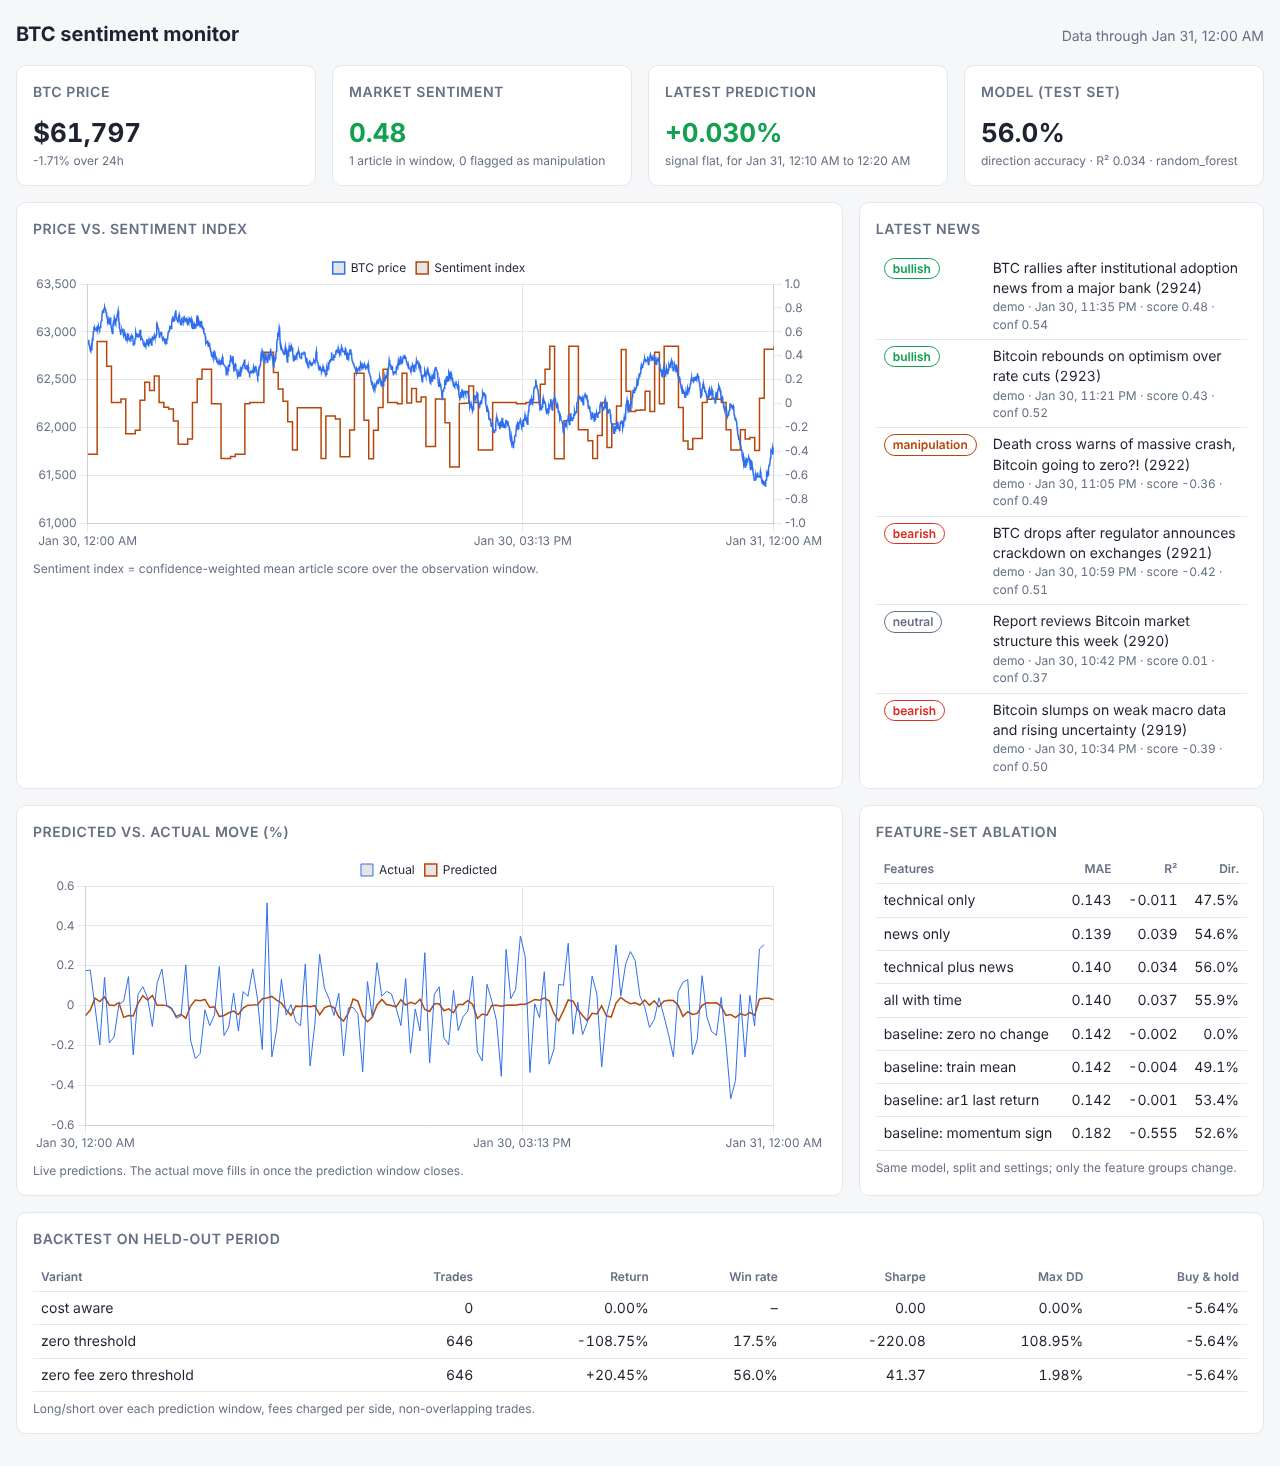
\includegraphics[width=0.72\linewidth]{figures/dashboard-demo.png}
  \caption{The system dashboard served by FastAPI.}
  \label{fig:dashboard}
\end{figure}

\UPDATE{Replace with a screenshot of the final dashboard (without the backtest table) if it has changed.}

\section{Comparison with the Original Report}
The earlier version of this project reported $R^2 = 0.83$ for the full model
against $R^2 = -0.02$ for technical features. Our rebuilt pipeline obtains
$R^2$ near zero for every feature set. We attribute the difference to the
evaluation fixes, not to worse features:
\begin{itemize}
  \item The original audit accepted news published \emph{during} the target
        window; ours requires all news to precede the target by at least 10
        minutes.
  \item Scaling, the correlation filter and noise were fitted on all data; ours
        are fitted inside each training fold.
  \item A single 70/15/15 split without an embargo let overlapping windows
        span the split; ours uses an embargo and walk-forward validation.
  \item Raw moving-average and Bollinger levels let trees memorise the price
        regime; ours are relative to price.
\end{itemize}
The original report itself listed the high $R^2$, the near-zero training
error and the dominance of counting features as warning signs. A near-zero
$R^2$ with above-chance direction accuracy is consistent with what is known
about intraday crypto returns.

\section{Limitations}\label{sec:limitations}
\begin{enumerate}
  \item \textbf{Short collection period.} Live collection started on 26
        November 2026, so the first run had \prelim{282} samples and a
        \prelim{7-hour} test period covering a single market regime.
  \item \textbf{Small test set.} Direction accuracies differ by a few
        correctly signed windows and their confidence intervals overlap.
  \item \textbf{No economic validation.} The fee-aware rule made no trades;
        transaction costs exceed the predicted moves at this horizon.
  \item \textbf{Single asset and source mix.} Results cover BTC/USDT on Binance
        and a particular set of English-language feeds, which changed during
        the first days as broken feeds were replaced.
  \item \textbf{LLM dependence.} Scores depend on one model version and prompt.
        The free tier imposes rate limits, and a retired model would change the
        scores.
  \item \textbf{Volume versus direction.} News volume follows working hours,
        so part of the news and time effect may be a time-of-day effect on
        volatility rather than sentiment direction.
\end{enumerate}

\UPDATE{Revise items 1 and 2 with the final period and sample sizes.}

% =====================================================================
\chapter{Conclusion}\label{ch:conclusion}
% =====================================================================

\section{Summary of Contributions}
\begin{itemize}
  \item \textbf{A working web mining system.} Live crawling of full-text news
        from CoinMarketCap and 30 RSS feeds, deduplication, Kafka streaming,
        LLM scoring within a free API tier, scheduled training and live
        predictions, all in one Docker Compose stack.
  \item \textbf{Richer LLM sentiment.} A prompt and JSON schema that return the
        label, score and confidence that the aggregation formulas require,
        with batching, fallbacks and safe key handling.
  \item \textbf{Leakage-safe evaluation.} An enforced 10-minute lag, a per-row
        audit, in-fold preprocessing, embargoed walk-forward validation and a
        single final holdout.
  \item \textbf{A first empirical answer.} On the first run, news features
        raised direction accuracy from \prelim{52\%} to \prelim{about 62\%}
        (\prelim{67\%} with time features) and the IC from \prelim{0.11} to
        \prelim{0.30--0.38}, with $R^2$ near zero.
\end{itemize}

\section{Critical Limitations}
The test set is small and covers one short period, the gains are not yet
statistically robust, and no profitable trading rule was found after
fees. See Section~\ref{sec:limitations}.

\section{Future Work}
\begin{itemize}
  \item Continue live collection for several weeks and evaluate on several
        non-overlapping test periods.
  \item Test longer horizons (e.g.\ \code{WINDOW_PRED_MIN=60}), where news
        effects are usually easier to detect and costs matter less.
  \item Separate sentiment direction from attention with ablations that use
        only counts or only scores.
  \item Compare Gemini with FinBERT \citep{araci2019finbert} and the lexicon on
        the same articles.
  \item Add social-media sources and other assets.
\end{itemize}

\section{Final Remarks}
The main lesson of this project is methodological. A pipeline that looks
very accurate can be measuring leakage, while a leakage-safe pipeline on
real 10-minute data gives modest, uncertain results. Our system makes the
honest version of the experiment easy to run and to repeat, and its first
results suggest that news sentiment carries some directional information
about short-term Bitcoin moves.

\UPDATE{Revise the last sentence after the final retrain if the conclusion changes.}

% =====================================================================
\appendix
\chapter{Appendix}\label{ch:appendix}
% =====================================================================

\section{Complete Feature Specifications}\label{sec:featlist}
\begin{longtable}{p{4.6cm}p{9.8cm}}
\caption{Technical features (21)}\label{tab:tech}\\
\toprule
\textbf{Feature} & \textbf{Description} \\
\midrule
\endfirsthead
\toprule
\textbf{Feature} & \textbf{Description} \\
\midrule
\endhead
\code{return_k}, $k\in\{1,2,3,5,10\}$ & Percentage return over the last $k$ minutes \\
\code{volatility_k}, $k\in\{5,10,20\}$ & Rolling std of 1-minute returns \\
\code{ma_k_ratio}, $k\in\{5,10,20\}$ & Price / $k$-minute moving average $-1$, in \% \\
\code{rsi_14} & Relative Strength Index, 14 periods (Wilder smoothing) \\
\code{macd}, \code{macd_signal}, \code{macd_histogram} & $(\mathrm{EMA}_{12}-\mathrm{EMA}_{26})/P$ in \%, its 9-period EMA, and their difference \\
\code{bb_upper_dist}, \code{bb_lower_dist} & Distance of the Bollinger bands ($\mathrm{MA}_{20}\pm2\sigma_{20}$) from price, in \% \\
\code{bb_width} & Band width relative to $\mathrm{MA}_{20}$, in \% \\
\code{log_volume}, \code{log_volume_ma5} & $\log(1+\text{volume})$ and of its 5-minute mean \\
\code{volume_ratio} & Volume / 5-minute mean volume \\
\bottomrule
\end{longtable}

\begin{longtable}{p{4.6cm}p{9.8cm}}
\caption{LLM sentiment features (16)}\label{tab:sentfeat}\\
\toprule
\textbf{Feature} & \textbf{Description} \\
\midrule
\endfirsthead
\toprule
\textbf{Feature} & \textbf{Description} \\
\midrule
\endhead
\code{sent_n_articles} & Articles in $\Wobs$ ($N$) \\
\code{sent_mean}, \code{sent_std} & Mean and std of scores $s_i$ \\
\code{sent_max}, \code{sent_min} & Most bullish and most bearish score \\
\code{sent_market} & Confidence-weighted score $S_{\mathrm{market}}$ \\
\code{sent_decay} & Recency- and confidence-weighted score $S_{\mathrm{decay}}$ \\
\code{sent_conf_mean} & Mean confidence $\bar{c}$ \\
\code{sent_n_manipulation} & Articles labelled manipulation \\
\code{sent_frac_*} & Share of bullish, bearish, neutral and manipulation labels (4 features) \\
\code{sent_velocity} & Share of the window's articles published in its last 10 minutes \\
\code{sent_n_articles_6h}, \code{sent_mean_6h} & Article count and mean score over the last 6 hours \\
\bottomrule
\end{longtable}

\begin{longtable}{p{4.6cm}p{9.8cm}}
\caption{NLP aggregate features (15)}\label{tab:nlpfeat}\\
\toprule
\textbf{Feature} & \textbf{Aggregation and description} \\
\midrule
\endfirsthead
\toprule
\textbf{Feature} & \textbf{Aggregation and description} \\
\midrule
\endhead
\code{pos_ratio}, \code{neg_ratio} & Mean share of positive and negative words \\
\code{compound} & Mean lexicon compound polarity \\
\code{word_count}, \code{sentence_count} & Sum over articles (attention) \\
\code{avg_sentence_length} & Mean tokens per sentence \\
\code{unique_word_ratio} & Mean vocabulary richness \\
\code{exclamation_count}, \code{question_count} & Sum of ``!'' and ``?'' \\
\code{btc_mention_count} & Sum of Bitcoin/BTC mentions \\
\code{price_keyword_count} & Sum of price words (surge, crash, rally, \ldots) \\
\code{technical_term_ratio} & Mean density of market jargon (ETF, liquidation, RSI, \ldots) \\
\code{hype_count} & Sum of hype phrases (``to the moon'', \ldots) \\
\code{ne_person_count}, \code{ne_org_count} & Sum of person and organisation entities \\
\bottomrule
\end{longtable}

\noindent\textbf{Time features (4):} \code{hour_sin}, \code{hour_cos},
\code{dow_sin}, \code{dow_cos}.

\section{Model Hyperparameters}\label{sec:hyper}
\begin{table}[H]
\centering
\caption{Model hyperparameters}
\label{tab:hyper}
\begin{tabularx}{\linewidth}{lY}
  \toprule
  \textbf{Model} & \textbf{Parameters} \\
  \midrule
  Ridge & $\alpha=10$, no noise injection \\
  Random forest & \code{n_estimators=300}, \code{max_depth=5}, \code{min_samples_split=10}, \code{min_samples_leaf=20}, \code{max_features='sqrt'} \\
  Gradient boosting & \code{n_estimators=200}, \code{learning_rate=0.05}, \code{max_depth=3}, \code{subsample=0.8}, \code{min_samples_leaf=30} \\
  LightGBM & \code{n_estimators=400}, \code{learning_rate=0.02}, \code{num_leaves=15}, \code{max_depth=4}, \code{min_child_samples=50}, \code{subsample=0.8}, \code{colsample_bytree=0.7}, \code{reg_lambda=5} \\
  All tree models & Gaussian noise 5\% of feature std (training only), \code{random_state=42} \\
  Pipeline & Median imputation, correlation filter $|r|>0.95$, min-max scaling, all fitted per fold \\
  \bottomrule
\end{tabularx}
\end{table}

\section{LLM Prompt}\label{sec:prompt}
The system prompt used for every article (\code{sentiment/prompt.py},
version v2). In batch mode up to ten articles are numbered and the schema is
an array of the object below.
\begin{lstlisting}
You are an expert cryptocurrency market analyst with 10 years of experience in
sentiment analysis and detecting market manipulation. Analyze the news article
below and judge its likely effect on the Bitcoin (BTC) price over the next hour.

Classify the article into exactly one category:

1. "manipulation": sensationalism, FOMO or FUD. Exaggerated price predictions
   ("skyrocket", "plummet", "to the moon", "death cross") without robust
   technical or fundamental backing, attempts to make readers buy or sell
   immediately, or paid promotion disguised as news.
2. "bullish": a reasonable, well-substantiated case that the BTC price may
   rise (on-chain data, institutional adoption, macro factors, ETF flows).
3. "bearish": a reasonable, well-substantiated case that the BTC price may
   fall (regulation, hacks, technical resistance, liquidations, macro).
4. "neutral": factual, objective reporting without a bullish or bearish stance.

If an article shows signs of both speculation and manipulation, choose
"manipulation" when the language is overly emotional or lacks evidence.

Also give:
- "score": a number from -1.0 (very bearish for BTC price) to 1.0 (very
  bullish). Use 0 for neutral. Manipulation articles still get a score in the
  direction they push readers (FOMO > 0, FUD < 0).
- "confidence": 0.0 to 1.0, how certain you are. Official, verifiable news
  (regulatory decisions, filings, exchange data) deserves high confidence;
  rumours and opinion pieces low confidence.
- "reasoning": one or two sentences citing specific phrases.

Return only JSON matching the schema.
\end{lstlisting}

\begin{lstlisting}[caption={Response schema (one article)},numbers=none]
{"label": "manipulation" | "bullish" | "bearish" | "neutral",
 "score": number, "confidence": number, "reasoning": string}
\end{lstlisting}

\begin{table}[H]
\centering
\caption{Gemini API configuration}
\label{tab:gemini}
\begin{tabular}{ll}
  \toprule
  \textbf{Parameter} & \textbf{Value} \\
  \midrule
  Model & \code{gemini-3.5-flash-lite} (free tier) \\
  Temperature & 0.2 \\
  Top-$p$ / top-$k$ & 0.8 / 40 \\
  Response format & JSON with response schema \\
  Articles per request & 10 \\
  Rate limit & 10 requests per minute \\
  Fallback & Other Flash model on 404; lexicon on repeated 503 \\
  \bottomrule
\end{tabular}
\end{table}

\section{Code Repository Structure}
\begin{lstlisting}[numbers=none]
src/cryptosent/
  collectors/  coinmarketcap.py, rss.py, gdelt.py, cryptocompare.py,
               prices.py (Binance), news_base.py (cleaning, dedup, crawling)
  sentiment/   prompt.py, gemini.py, lexicon.py, finbert.py, nlp_features.py
  features/    technical.py, sentiment_agg.py, dataset.py (builder + audit)
  models/      registry.py, train.py (protocol), evaluate.py, baselines.py
  api/         app.py (FastAPI) + static/index.html (dashboard)
  pipeline.py  tasks shared by the CLI, DAGs and services
  streaming.py Kafka producer and sentiment consumer
  storage.py   MongoDB and local storage
airflow/dags/  cryptosent_dags.py
docker/        app and Airflow images
tests/         unit and end-to-end tests
report/        this report (main.tex, refs.bib, figures/)
\end{lstlisting}

\section{Experimental Environment}
\begin{table}[H]
\centering
\caption{Experimental environment}
\label{tab:env}
\begin{tabular}{ll}
  \toprule
  \textbf{Component} & \textbf{Version / specification} \\
  \midrule
  Machine & Windows 11 laptop, 16 GB RAM \\
  Containers & Docker Desktop with WSL2, 8 GB assigned \\
  Python & 3.10+ \\
  Key libraries & pandas 2, scikit-learn 1.4+, LightGBM 4, NLTK 3.8+ \\
  Services & MongoDB 7.0, Kafka 3.8, Airflow 2, MLflow 2.17, FastAPI \\
  LLM & Google Gemini \code{gemini-3.5-flash-lite} \\
  \bottomrule
\end{tabular}
\end{table}

\TOFILL{Check the exact Airflow and library versions in the running containers (\code{pip list}).}

\section{Reproducing the Results}
\begin{lstlisting}[numbers=none]
cp .env.example .env            # add GEMINI_API_KEY
docker compose up -d --build    # start the stack
# Airflow UI: trigger backfill_history once (90 days of prices)
# after collection, trigger train_daily, or run inside the app container:
cryptosent train
# results: artifacts/report.md, report.json, test_predictions.csv, MLflow
\end{lstlisting}

\bibliographystyle{plainnat}
\bibliography{refs}

\end{document}
